\documentclass{article}
\usepackage{tikz}
\usetikzlibrary{positioning}

\begin{document}
\begin{center}
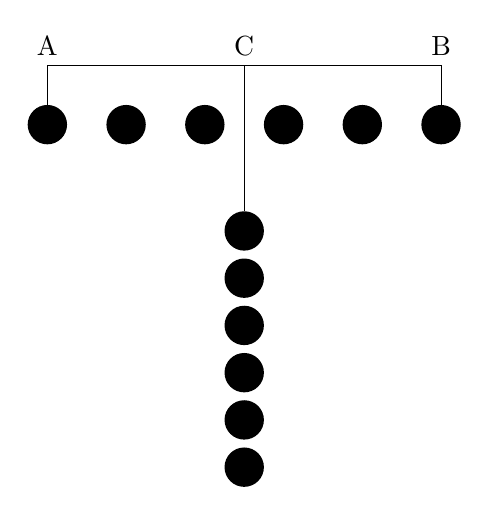
\begin{tikzpicture}
% definizione colore di riempimento
\tikzset{myfillcolor/.style ={fill=#1, draw=none}}
% definizione delle caratteristiche del nodo
\tikzset{mynode/.style={rectangle,draw, minimum width=0.5cm, minimum height=0.5cm}}
%forse preferisci pesi circolari
\tikzset{mynode/.style={circle,draw, minimum width=0.5cm, minimum height=0.5cm}}

%----
% inserimento nodi orizzontali
\foreach \x in {0.5,1.5,...,5.5}
\node[mynode,myfillcolor=black] at (\x,0.75) {};
% inserimento nodi vertical
\foreach \y in {-0.6,-1.2,...,-3.6}
\node[mynode,myfillcolor=black]at (3,\y) {};

% inserimento path che collega i primi due nodi orizzontali
\draw (0.5,0.75)--(0.5,1.5)--(5.5,1.5)--(5.5,0.75);
% inserimento label A B C
\foreach \t/\text in {{(0.5,1.5)/A},{(3,1.5)/C},{(5.5,1.5)/B}}
\node[above]at \t {\text};

% inserimento path che collega C con i nodi verticali
\draw (3,1.5)--(3,-0.35);
\end{tikzpicture}
\end{center}
\end{document}
